%======================================================================
\section{Supresión de movimiento: el peso $R$ (F8)}\label{sec:supresion}
%======================================================================
La formulación de los lazos cerrados (sección~\ref{sec:formulacion-final}) no pone ningún
peso sobre los cambios del caudal: entre dos caudales que dan la misma PCT predicha, el costo
no prefiere el más suave. En MPC lo habitual es agregar la \emph{supresión de movimiento}
\[
J_R(u)=J(u)+R\sum_{k=1}^{K}(u_k-u_{k-1})^2,
\]
con $u_0$ el caudal aplicado en la consulta anterior. A diferencia de la rampa, que es un
límite del actuador, $R$ expresa una preferencia: menos desgaste y transitorios de presión
más suaves, la razón que en 2025 justificó la rampa. Con $R=0$ se recupera la formulación de
F5--F7.

\paragraph{Campaña.} Once valores, $R\in\{0,\,10^{-3},\,10^{-2},\,0.03,\,0.1,\,0.3,\,1,\,3,\,10,\,30,\,100\}$
K$^2$/(kg/s)$^2$, en tres pruebas:
(i) lazo con fallas del DET (familia det, 50 realizaciones, N2 con sesgo; N3 en
$R\in\{0,0.1,10\}$); (ii) familia nominal (50 realizaciones, N2); (iii) lazo sin fallas con el
estimador de Rao--Blackwell (sección~\ref{sec:riesgo-rb}), N2 sin y con la cota de riesgo
$\alpha=0.02$.
Son 2350 lazos a 40~kg/s, con la rampa dura de 5~kg/s por paso, en 26~min en Olab
(\code{julia/F6Tasks.jl}, campañas \code{rmove} y \code{rrisk}; \code{python/f8\_rmove.py};
\code{results/f8\_rmove/}).

\subsection{La curva seguimiento--suavidad}
La figura~\ref{fig:f8-tradeoff} es la frontera que $R$ recorre. Con $R$ pequeño, el caudal
se suaviza casi gratis. Pasado $R\approx1$, cada reducción de la variación total cuesta mucho
seguimiento.

\begin{figure}[H]\centering
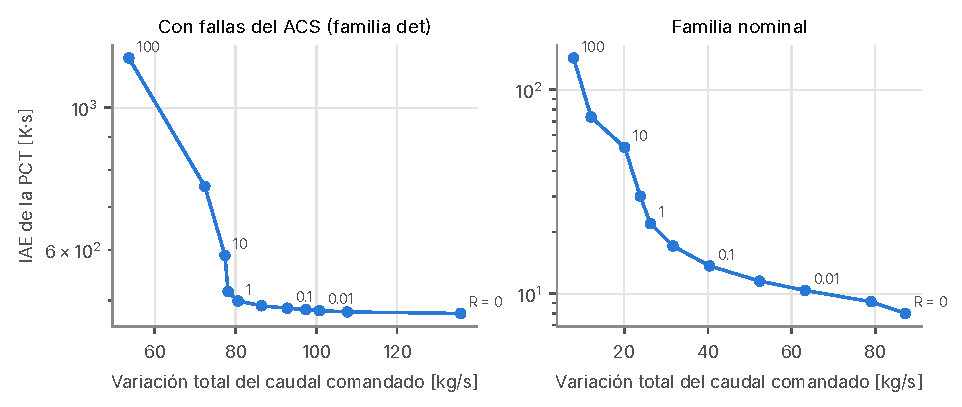
\includegraphics[width=\linewidth]{figures/fig_f8_tradeoff.pdf}
\caption{IAE de la PCT frente a la variación total del caudal mandado, promedio de 50
realizaciones por punto, un punto por valor de $R$. Izquierda: con fallas del DET, donde el IAE
lo dominan las fallas. Derecha: familia nominal.}
\label{fig:f8-tradeoff}
\end{figure}

\begin{table}[H]\centering\small
\begin{tabularx}{\linewidth}{@{}c Y Y Y Y c@{}}\toprule
$R$ & IAE nominal [K\,s] & VT nominal [kg/s] & IAE det [K\,s] & VT det [kg/s] & det: cruzan 1220~K\\\midrule
0 & 8.0 & 87 & 477 & 136 & 0/50\\
0.01 & 10.4 & 63 & 482 & 101 & 0/50\\
0.1 & 13.7 & 40 & 486 & 93 & 0/50\\
1 & 22.1 & 26 & 499 & 81 & 0/50\\
10 & 52.1 & 20 & 588 & 77 & 0/50\\
100 & 143 & 7.9 & 1196 & 54 & 2/50\\\bottomrule
\end{tabularx}
\caption{Seguimiento y suavidad según $R$ (promedios de 50 realizaciones). Las diferencias
pareadas contra $R=0$ excluyen el cero en todos los casos (\code{results/f8\_rmove/summary.md}).}
\label{tab:f8}
\end{table}

\begin{itemize}
  \item \textbf{Familia nominal.} $R=0.1$ reduce la variación total 54\,\% (de 87 a 40~kg/s), y
        el IAE pasa de 8.0 a 13.7~K\,s. Con $R=100$ el controlador ya no llega a la consigna: la
        PCT queda al menos 1.7~K sobre ella en todo el lazo.
  \item \textbf{Con fallas.} El IAE lo dominan las fallas. Con $R$ entre 0.1 y 1 cambia en menos de
        5\,\%, y la variación total baja un 32--41\,\%. Con $R=30$ y $R=100$, una y dos
        realizaciones cruzan 1220~K, contra ninguna con $R=0$: un controlador lento recupera
        peor tras una falla.
  \item \textbf{N3 y N2 siguen coincidiendo.} Con el mismo $R$, las trayectorias de PCT de N3 y
        N2 difieren en $\le0.002$~K y los caudales en $\le0.026$~kg/s ($R\in\{0,0.1,10\}$, 50
        pares). La equivalencia certificada en la sección~\ref{sec:f7} se
        extiende a $R>0$.
\end{itemize}

\subsection{La capa de riesgo oscilaba, y $R$ lo corrige sin costo}
Las capas de riesgo de F6 tienen una variación total de 1450 a 1920~kg/s, entre 11 y 22 veces la
de N2 (tabla~\ref{tab:det-tesis}). La causa es una oscilación de período dos: en una
realización típica (semilla 201, cota $\alpha=0.02$), el caudal alterna
$12\leftrightarrow17$~kg/s, a la rampa máxima, en 280 de 480 pasos. La oscilación llega a la
planta: la variación total del caudal recibido es la misma que la del mandado.

\begin{figure}[H]\centering
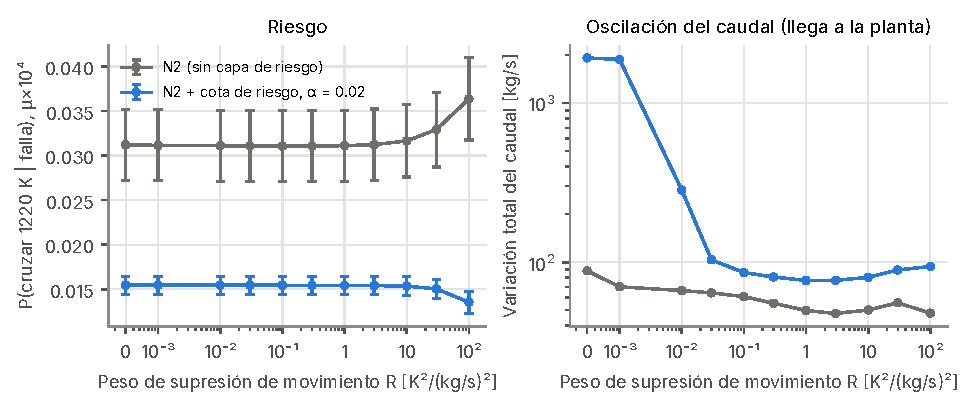
\includegraphics[width=\linewidth]{figures/fig_f8_risk.pdf}
\caption{Izquierda: probabilidad de cruzar 1220~K dada una falla (Rao--Blackwell, $\mu\times10^4$,
50 realizaciones, IC al 95\,\%). Derecha: variación total del caudal. Con la cota de riesgo, desde
$R=0.03$ la oscilación desaparece y el riesgo no cambia.}
\label{fig:f8-risk}
\end{figure}

\noindent Con $R\ge0.03$ la oscilación desaparece (figura~\ref{fig:f8-risk}). Con $R=0.1$, la
variación total baja de 1923 a 86~kg/s, al nivel de N2. Lo demás no cambia: la probabilidad
de cruce pasa de 0.01545 a 0.01544, el preenfriamiento sigue en 7.4~K, la masa inyectada en
4337~kg y el IAE en $\approx1820$~K\,s. Una explicación probable: con la cota activa, el
costo es casi plano en la dirección del primer movimiento (la penalización $\ell_1$ exacta
tiene un quiebre en la cota, y el sesgo $d$ se reestima en cada consulta), así que el solver
cambia de solución de una consulta a otra sin pagar nada. $R>0$ vuelve el costo
estrictamente convexo en $\Delta u$ y elige la solución suave. Las conclusiones de riesgo de
las secciones~\ref{sec:prop-aditiva}--\ref{sec:riesgo-aplicabilidad} se mantienen, porque
probabilidad, margen y masa no dependen de la oscilación. Lo que cambia es la recomendación:
el controlador con capa de riesgo debe llevar un $R$ pequeño.

\paragraph{Sin capa de riesgo,} $R$ casi no mueve el riesgo hasta $R\approx3$
(P = 0.0312). Con $R=100$ sube a 0.0364 (+16\,\%): el controlador suave sigue con retraso la
deriva de la fuga y la PCT queda en promedio 0.4~K sobre la consigna, con menos margen ante la
falla. Con la cota de riesgo ocurre lo contrario: la cota obliga a preenfriar, y un controlador
más lento preenfría más (9.3~K con $R=100$), con lo que el riesgo baja a 0.0135.

\paragraph{Verificación de la proposición~\ref{prop:blanda-dura}.} En esta campaña se registró
además la PCT \emph{predicha} máxima del plan aplicado en cada consulta. En los 2350 lazos es
1220.32~K, a 23.7~K de $U_y$. La penalización del margen no se activa en ninguna consulta, y
por lo tanto la versión blanda y la dura coinciden también sobre la predicción, no sólo sobre
la PCT de la planta.

\takeaway{\textbf{Supresión de movimiento.} $R$ recorre una frontera seguimiento--suavidad con
un codo en $R\approx0.1$--1. Su efecto más útil está en la capa de riesgo: con $R\ge0.03$
desaparece una oscilación de período dos del caudal, que llegaba a la planta, sin cambiar
el riesgo, el margen ni la masa. Se propone $R=0.1$ para el controlador del paper.}
